\section{Results}\label{sec:results}
Four circuits were assembled and analyzed using a function generator to apply a stimulus sinusoid of 1\si{\voltpp} at 1\si{\kilo\hertz}, and an oscilloscope to measure the output of the system. Circuit schematics are taken from the lab manual \cite{lab-manual}.

\begin{figure}[htbp]
	\centering
	\subfigure[$R_1=R=\SI{10}{\kilo\ohm}$]
	{
		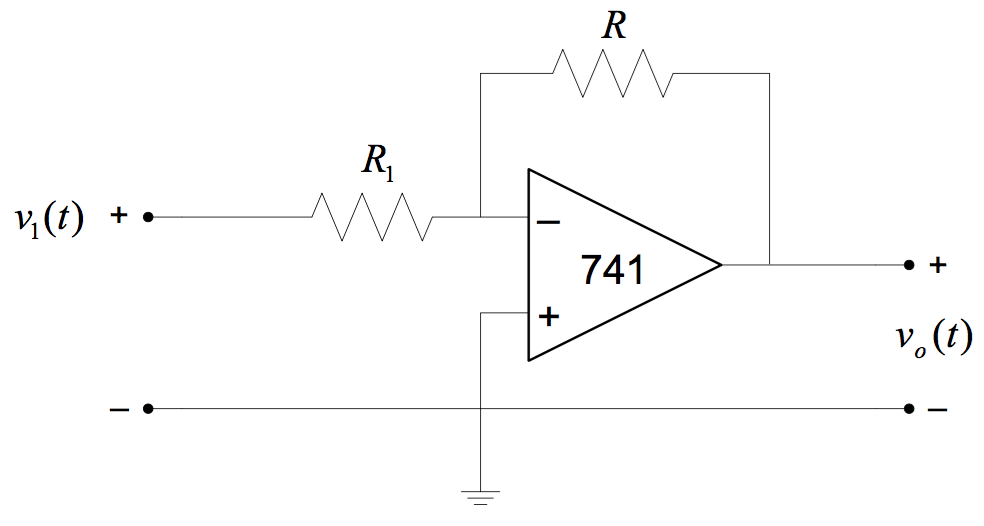
\includegraphics[width=0.475\linewidth]{schematic-inverter}
	}
	\subfigure[$V_o$, top; $V_i$, bottom]
	{
		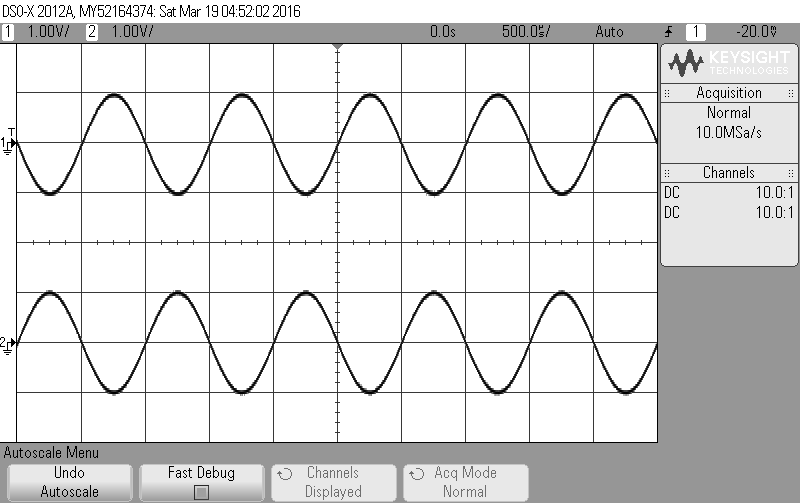
\includegraphics[width=0.475\linewidth]{response-inverter}
	}
	\label{fig:inverter}
	\caption{Inverter}
\end{figure}

\begin{figure}[htbp]
	\centering
	\subfigure[$R=R_1=R_2=\SI{10}{\kilo\ohm}$]
	{
		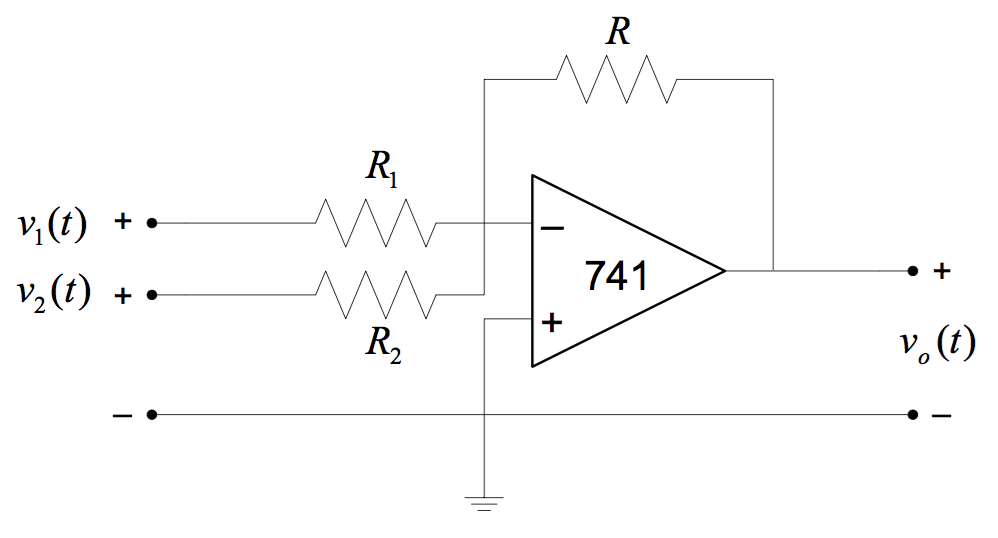
\includegraphics[width=0.475\linewidth]{schematic-adder}
	}
	\subfigure[$V_o$, top; $V_i$, bottom]
	{
		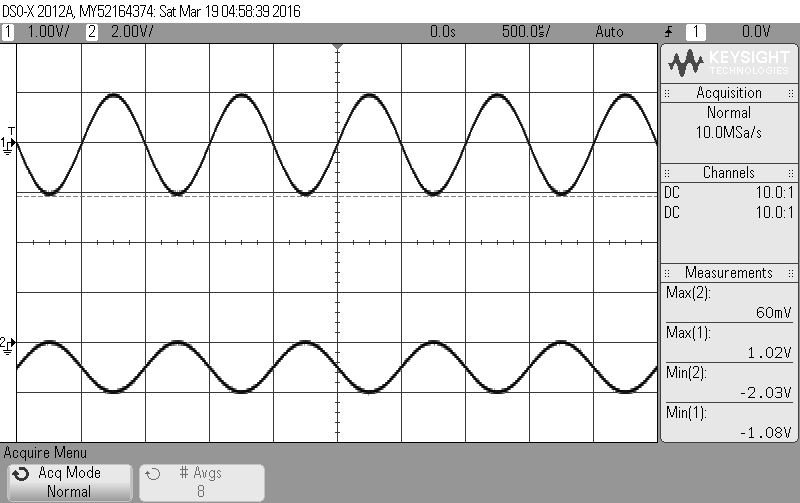
\includegraphics[width=0.475\linewidth]{response-adder}
	}
	\label{fig:adder}
	\caption{Adder}
\end{figure}

\begin{figure}[htbp]
	\centering
	\subfigure[$C=\SI{16}{\nano\farad}$, $R_1=\SI{10}{\kilo\ohm}$]
	{
		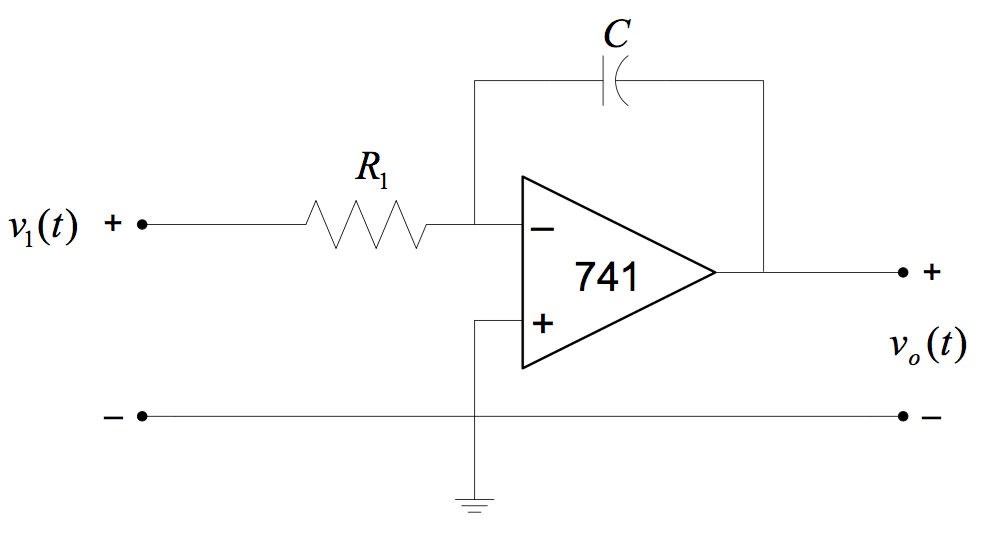
\includegraphics[width=0.475\linewidth]{schematic-integrator}
	}
	\subfigure[Rising edge of $V_o$]
	{
		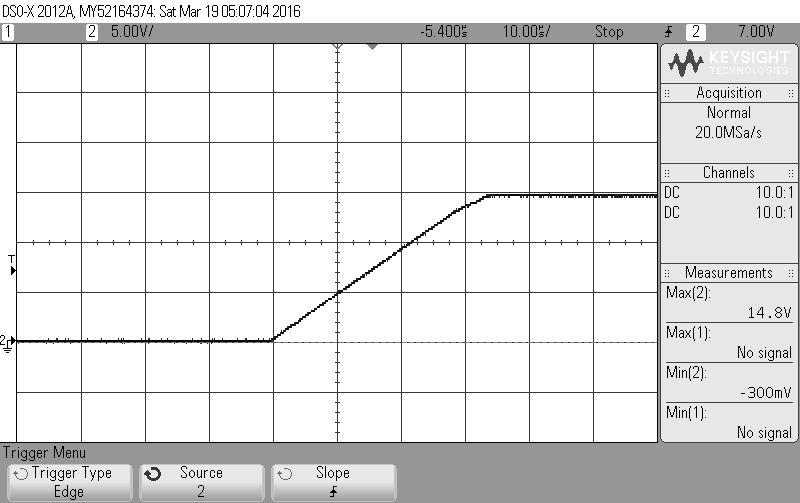
\includegraphics[width=0.475\linewidth]{response-integrator}
	}
	\label{fig:integrator}
	\caption{Integrator}
\end{figure}

\begin{figure}[htbp]
	\centering
	\subfigure[$C=\SI{16}{\nano\farad}$, $R_1=R_2=\SI{10}{\kilo\ohm}$]
	{
		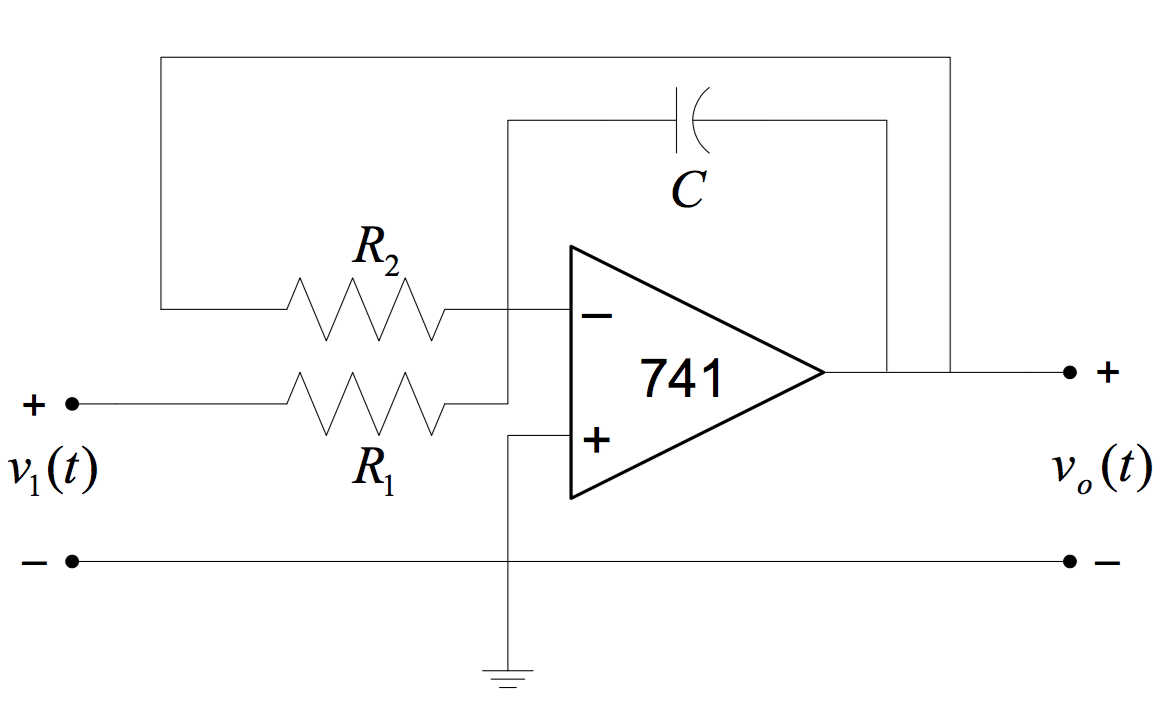
\includegraphics[width=0.475\linewidth]{schematic-first-order}
	}
	\subfigure[$V_i$, top; $V_o$, bottom]
	{
		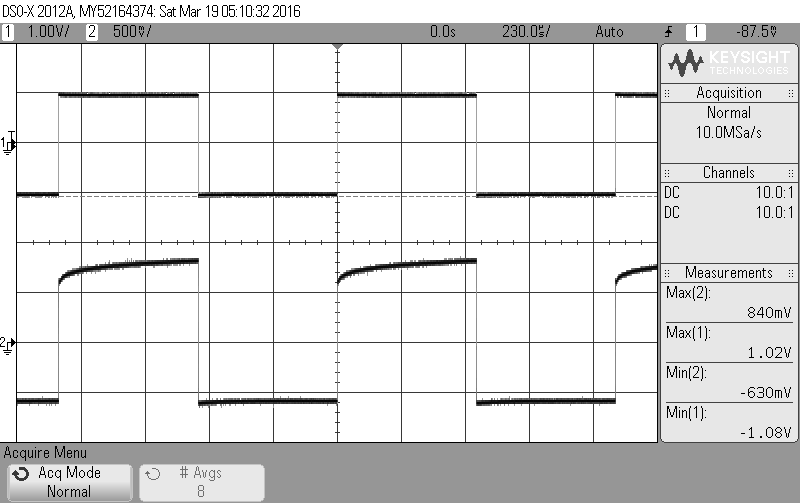
\includegraphics[width=0.475\linewidth]{response-first-order}
	}
	\label{fig:first-order}
	\caption{Integrator as a first order system with feedback}
\end{figure}

\clearpage
